\section{When does aggregation pay?}\label{sec:pay}

Fewer iterations are not the same as less work. This section separates
the two: an exact expression for how much more progress a block makes
than the single MDM step at the same iterate, a cost model for what the
block costs, a theorem that bounds the drop steps by an identification
phase rather than by the crude count of Theorem~\ref{thm:linear}, and
measurements of every quantity in the model on the five real cells of
Section~\ref{sec:exp}.

\subsection{Progress per unit of work at one iterate}

Consider a case-(a) iteration with $k'$ retained pairs, all uncapped,
so that $\gamma_j=\mathrm{gap}_j/\norm{d_j}^2$ and pair $j$ alone would
gain $\Delta_j=\mathrm{gap}_j^2/(2\norm{d_j}^2)$, with $\Delta_1$ the MDM
gain. Write
\[
Q=\frac{\sum_{j\le k'}\Delta_j}{\Delta_1},\qquad
\chi=\frac{D}{S},\qquad
S=\sum_j\gamma_j\mathrm{gap}_j=2\sum_j\Delta_j,\qquad
D=\Big\lVert\sum_j\gamma_jd_j\Big\rVert^2 .
\]
$Q$ measures how much useful progress the block has beyond its leading
pair and $\chi$ how much the directions lose (or gain) by being
combined; orthogonal directions give $\chi=1$. Call the block
\emph{$\eta$-diverse} if $|\ip{d_i}{d_j}|\le\eta\norm{d_i}\norm{d_j}$ for
$i\ne j$ and \emph{$\beta_{\mathrm{flat}}$-flat}, $0<\beta_{\mathrm{flat}}\le1$, if
$\Delta_j\ge\beta_{\mathrm{flat}}\Delta_1$ for every $j$ (the subscript keeps
the flatness parameter apart from the $W$-side weights $\beta$).

\begin{proposition}[Exact gain ratio]\label{prop:ratio}
At such an iteration the exact line search gives
\[
\frac{\Delta_B}{\Delta_1}=Q\cdot\begin{cases}2-\chi,&\chi\le1,\\
1/\chi,&\chi\ge1.\end{cases}
\]
If the block is $\eta$-diverse then $\chi\le1+\eta(k'-1)$; if it is
$\beta_{\mathrm{flat}}$-flat then $Q\ge1+\beta_{\mathrm{flat}}(k'-1)$; hence the guarded step gains at
least
\[
\max(\Delta_B,\Delta_1)\ \ge\ \Delta_1\,\frac{1+\beta_{\mathrm{flat}}(k'-1)}{1+\eta(k'-1)} .
\]
\end{proposition}
\begin{proof}
For uncapped pairs $\gamma_j\norm{d_j}^2=\mathrm{gap}_j$, so
$S=\sum_j\mathrm{gap}_j^2/\norm{d_j}^2=2\sum_j\Delta_j$ and
$\varphi_j^2=\gamma_j^2\norm{d_j}^2=\gamma_j\mathrm{gap}_j$, whence
$\sum_j\varphi_j^2=S$. The line search takes $\theta=\min(S/D,1)$. If $D\ge S$
the optimum is interior and $\Delta_B=S^2/(2D)=(S/2)/\chi=\sum_j\Delta_j/\chi$;
if $D<S$ then $\theta=1$ and $\Delta_B=S-D/2=(S/2)(2-\chi)$. Dividing
by $\Delta_1$ gives the two cases. For the bound on $\chi$,
$D=\sum_{i,j}\gamma_i\gamma_j\ip{d_i}{d_j}\le\sum_j\varphi_j^2+\eta\sum_{i\ne j}\varphi_i\varphi_j
\le(1+\eta(k'-1))\sum_j\varphi_j^2=(1+\eta(k'-1))S$ by Cauchy--Schwarz on the
cross terms; flatness gives $\sum_j\Delta_j\ge\Delta_1(1+\beta_{\mathrm{flat}}(k'-1))$.
When $\chi\le1$ the ratio is $Q(2-\chi)\ge Q$, and when $\chi\ge1$
it is $Q/\chi$; both are at least the stated bound.
\end{proof}
Proposition~\ref{prop:ratio} recovers the diversity bound of Proposition~\ref{prop:orth} and adds the comparison with $\Delta_1$. The two
numbers $Q$ and $\chi$ are computed by the guard at every block step
(from $S$, $D$ and the per-pair gaps), so both are observable at no
extra cost. Note the direction of the inequalities: the theorem's $\eta$
bounds the \emph{maximum} absolute pairwise cosine of the retained
directions, whereas the \emph{effective correlation}
\[
\hat\eta:=\frac{\chi-1}{k'-1}\qquad(k'>1)
\]
that a block step reveals is a $\gamma$-weighted aggregate in which
cross terms can cancel; the proof gives $\hat\eta\le\eta$, and $\hat\eta$
can be negative. Likewise $Q/k'$ close to $1$ says the average pair is
as good as the leading one, not that every pair is ($\beta_{\mathrm{flat}}$-flatness).
The empirical model of Section~\ref{sec:pay-meas} is therefore stated in
$Q$ and $\chi$, the quantities the guard measures, and the theorem's
assumptions (all retained pairs uncapped, maximum cosine at most $\eta$,
minimum relative gain at least $\beta_{\mathrm{flat}}$) are recorded separately.

\paragraph{Cost.} Per iteration the solver pays a scan and certificate
cost that does not depend on $k$, a step cost that grows with the number
of retained pairs (the $k'$-column score update and the $O(k'^2)$ guard), and one Gram or kernel column for every
receiver or donor not in the cache. Write
\[
\mathcal C_B=a+b\,k'+c_{\mathrm{col}}\,n^{\mathrm{new}}_B,\qquad \mathcal C_1=a+b+c_{\mathrm{col}}\,n^{\mathrm{new}}_1,
\]
for the block and the single step from the same state, where $n^{\mathrm{new}}_B\ge n^{\mathrm{new}}_1$
count the column misses of the two candidates ($n^{\mathrm{new}}_1\le1$: only the MDM
receiver can be new) and $a,b,c_{\mathrm{col}}$ are timing coefficients.
They are fitted, not assumed: they depend on $n$, $d$, the
representation (dense, kernel) and the hardware, and
Section~\ref{sec:pay-meas} fits them per cell. The model is a timing
approximation of the implementation, not an upper bound on
computational work. The guarded block improves progress per unit of work at this
iterate exactly when
$\max(\Delta_B,\Delta_1)/\Delta_1>\mathcal C_B/\mathcal C_1$; by
Proposition~\ref{prop:ratio} a sufficient condition is
\begin{equation}\label{eq:ppc}
\frac{1+\beta_{\mathrm{flat}}(k'-1)}{1+\eta(k'-1)}\;>\;\frac{a+bk'+c_{\mathrm{col}}n^{\mathrm{new}}_B}{a+b+c_{\mathrm{col}}n^{\mathrm{new}}_1}.
\end{equation}
Two regimes are visible in \eqref{eq:ppc}. If $c_{\mathrm{col}}$
dominates $a$ and $b$, the right-hand side is governed by the miss
counts: the block loses when it touches more new points than the single
step ($n^{\mathrm{new}}_B>n^{\mathrm{new}}_1$) and can still win by the full gain ratio when both
need the same column ($n^{\mathrm{new}}_B=n^{\mathrm{new}}_1$), so column dominance limits the gain
to the iterations on which the block's extra receivers are cached; it
does not exclude it. If the per-iteration terms dominate, the
right-hand side is $(a+bk')/(a+b)$, linear in $k'$, while the left-hand
side saturates at $\beta_{\mathrm{flat}}/\eta$; the ratio of the two is maximised at
\begin{equation}\label{eq:kstar}
k^*=\sqrt{\frac{a(1-\eta)}{b\,\eta}}\qquad(\beta_{\mathrm{flat}}=1),
\end{equation}
the block size at which the marginal cost of one more pair equals its
marginal gain. Equation~\eqref{eq:kstar} is the unconstrained continuous
optimiser of the model for $a,b>0$ and $0<\eta<1$: as $\eta\to0$ it grows
without bound (every pair helps), as $\eta\to1$ it tends to $0$ (only the
leading pair helps), and an implementation rounds it and clips it to
$\{1,\dots,k_{\max}\}$.

\subsection{Drops are an identification cost}

Theorem~\ref{thm:linear} charges up to $k$ drop steps per non-drop
iteration, which would cancel a $k$-fold gain in progress. The
measurements below show that drops in fact happen while the support is
being built and stop once it has settled. The following theorem proves
this under the standard non-degeneracy assumptions of active-set
identification \citep{bomze2020,garber2020}: after an explicit
iteration, every step that removes a non-face point is a drop, no
non-face point enters, and once the supports lie in the optimal faces
and the weights are close to the optimal ones, no step is a drop at all.

Write $\mathcal F_V=\conv\{v_i:i\in F_V\}$ and
$\mathcal F_W=\conv\{w_j:j\in F_W\}$ for the geometric faces ($F_V,F_W$
remain index sets), and let $V_{F_V}\in\R^{d\times|F_V|}$,
$W_{F_W}\in\R^{d\times|F_W|}$ be the matrices whose columns are the face
points. A witness pair $(p^*,q^*)$ with $p^*=\sum_i\alpha^*_iv_i$,
$q^*=\sum_j\beta^*_jw_j$ and $p^*-q^*=z^*$ carries optimal weights
$\alpha^*,\beta^*$.
\begin{assumption}\label{ass:nondeg}
(A1) \emph{Strict complementarity}: $F_V=\operatorname{supp}\alpha^*$ and
$F_W=\operatorname{supp}\beta^*$, and
$\alpha_{\min}:=\min\big(\min_{i\in F_V}\alpha^*_i,\ \min_{j\in F_W}\beta^*_j\big)>0$
is the smallest positive optimal weight over both classes. (A2)
\emph{Non-degeneracy}: the witness pair $(p^*,q^*)$ is unique, the
vertices of each optimal face are affinely independent (so
$\alpha^*,\beta^*$ are unique), and $\sigma>0$ denotes a constant with
$\norm{\alpha-\alpha^*}_1+\norm{\beta-\beta^*}_1\le\norm{(p-q)-z^*}/\sigma$
for all $p\in\mathcal F_V$, $q\in\mathcal F_W$ with face weights
$\alpha,\beta$ (such a constant exists under the two preceding
conditions and is computed below). Let $d_{\min}>0$ be the smallest distance from a face
vertex to the affine hull of the other vertices of its face, the minimum
taken over the faces with at least two points; if both faces are
singletons, $(p^*,q^*)$ is the unique pair of face points and the
no-drop conclusions below hold as soon as the supports lie in the faces.
\end{assumption}
Affine independence and uniqueness of the witness pair make the linear
map $(\alpha-\alpha^*,\beta-\beta^*)\mapsto(p-q)-z^*$ injective on the
subspace $U=\{\sum_i(\alpha_i-\alpha^*_i)=0=\sum_j(\beta_j-\beta^*_j)\}$
of $\R^{|F_V|+|F_W|}$; if $\sigma_2>0$ is the smallest singular value of
$[V_{F_V},-W_{F_W}]$ restricted to $U$, then
$\sigma=\sigma_2/\sqrt{|F_V|+|F_W|}$ works, the square root being the
conversion from the Euclidean to the $\ell_1$ norm of the weights. When
$U=\{0\}$ (both faces singletons) any $\sigma>0$ works and the weight
condition is void.

Recall $\varrho_t=\sqrt{\UB^2-\max(\LB,0)^2}\ge\norm{z_t-z^*}$ and, from the
proof of Theorem~\ref{thm:activation}, $\varrho_t^2\le(4R^2/\delta^*)\sqrt{2h_t}$,
so that $\varrho_t\le c$ whenever $h_t\le c^4\delta^{*2}/(32R^4)$. Let
$\ell_t$ be the total support size, $\zeta_k=k+1$ (one-sided) or $2k+1$
(two-sided schedule), and define
\begin{align*}
H_{\mathrm{id}}&=\min\Big\{\frac{\tau^4\delta^{*2}}{41472\,R^4L^4},\ \frac{\tau^2}{12L^2},\ \frac{\tau}{12},\ h_3\Big\},\qquad
h_3=\max\{h:\ 2h+R\sqrt{2h}\le\tau/6\},\\
H_{\mathrm w}&=\min\Big\{H_{\mathrm{id}},\ \frac{(\sigma\alpha_{\min}/2)^4\delta^{*2}}{32R^4},\
\frac{(\alpha_{\min}d_{\min}^2/(2L))^4\delta^{*2}}{32R^4}\Big\}.
\end{align*}

\begin{theorem}[Identification and drop count]\label{thm:ident}
Let $\delta^*>0$, let $\tau,L,R$ be as in Theorem~\ref{thm:activation}
and let the guarded block-transfer algorithm run with any $k\ge1$ under
either schedule of Theorem~\ref{thm:linear}. Let $t_{\mathrm{id}}$ be the
first iteration with $h_t<H_{\mathrm{id}}$ and $N$ the number of
non-face support indices at $t_{\mathrm{id}}$.
\begin{enumerate}\setlength\itemsep{0pt}
\item[(i)] For every $t\ge t_{\mathrm{id}}$: if either side's support
contains a non-face point, the step taken is a drop of a non-face point;
and no non-face point enters either support. Hence
$\operatorname{supp}\alpha\subset F_V$ and $\operatorname{supp}\beta\subset F_W$
from iteration $t_{\mathrm{id}}+N$ on, and
$N\le \ell_{t_{\mathrm{id}}}\le \ell_0+\zeta_k\,t_{\mathrm{id}}$.
\item[(ii)] Under Assumption~\ref{ass:nondeg}, let $t_{\mathrm w}$ be the
first iteration with $h_t<H_{\mathrm w}$. No iteration
$t\ge\max(t_{\mathrm w},t_{\mathrm{id}}+N)$ is a drop, and no block pair
is capped at such an iteration. Consequently every drop occurs before
$t_{\mathrm w}+N$, the number of drops is at most
$\zeta_k(t_{\mathrm w}+N)+\ell_0$, and
$t_{\mathrm w}\le \ell_0+1+\tfrac{\zeta_k}{\rho}\log\max\{1,h_0/H_{\mathrm w}\}$.
\item[(iii)] For $t\ge\max(t_{\mathrm w},t_{\mathrm{id}}+N)$ every
iteration contracts. Let $\rho^{\mathrm{act}}_t:=1-h_{t+1}/h_t$ (for
$h_t>0$) be the actual contraction and, for $j\ge1$,
\[
\underline\rho_j:=\min\Big\{1,\ 4\rho\max\Big[1,\frac{1+\beta_{\mathrm{flat}}(j-1)}{1+\eta(j-1)}\Big]\Big\},
\]
which is nondecreasing in $j$. Then $\rho^{\mathrm{act}}_t\ge\rho$, and
$\rho^{\mathrm{act}}_t\ge\underline\rho_{k'}$ when the iteration is case
(a) with an $\eta$-diverse, $\beta_{\mathrm{flat}}$-flat block of $k'$
pairs (under the two-sided schedule, the block of the first,
larger-gap side, which is the step the progress argument uses).
\end{enumerate}
\end{theorem}

\begin{proof}
Throughout, $s_i=\ip{g}{v_i}=-\ip{z}{v_i}$ on side $V$ and
$s_j=\ip{z}{w_j}$ on side $W$; we argue on side $V$, side $W$ being
symmetric with the maximum in place of the minimum.

\emph{Three facts.} (F1) If $\varrho\le\tau/(6L)$ then for $i\notin F_V$ and
$j\in F_V$,
$s_j-s_i=\ip{z}{v_i-v_j}=\ip{z^*}{v_i-v_j}+\ip{z-z^*}{v_i-v_j}\ge\tau_i-\varrho L\ge5\tau/6$,
while for $i,j\in F_V$, $|s_i-s_j|\le\varrho L\le\tau/6$; in particular the
global argmax of $s$ is a face point. (F2) Let $\omega_t$ be the total
weight on non-face points of both sides. By convexity
$h_t\ge\ip{\nabla F(z^*)}{z_t-z^*}=\ip{z^*}{z_t-z^*}$; writing
$\vartheta_V:=\min_i\ip{z^*}{v_i}$ and $\vartheta_W:=\max_j\ip{z^*}{w_j}$, so that
$\ip{z^*}{v_i}=\vartheta_V+\tau_i$ and $\ip{z^*}{w_j}=\vartheta_W-\tau_j$, and using
$\norm{z^*}^2=\ip{z^*}{p^*-q^*}=\vartheta_V-\vartheta_W$ (the optimal weights live on the
faces, where the margins vanish),
$\ip{z^*}{z_t-z^*}=\sum_i\alpha_i\tau_i+\sum_j\beta_j\tau_j\ge\tau\,\omega_t$.
Hence $\omega_t\le h_t/\tau$. (F3) By the radius bound quoted above,
$h_t<H_{\mathrm{id}}$ implies $\varrho_t\le\tau/(6L)$, $\omega_t\le\tau/(12L^2)$,
$\omega_t\le1/12$ and $2h_t+R\sqrt{2h_t}\le\tau/6$.

\emph{(i) Identification.} Let $h_t<H_{\mathrm{id}}$ and suppose
$\operatorname{supp}\alpha\not\subset F_V$. The worst active donor $u$
minimises $s$ over the support, so by (F1) $u\notin F_V$. The away gap of
side $V$ is $\gA_V=\sum_i\alpha_i(s_i-s_u)\ge\sum_{i\in F_V}\alpha_i\cdot5\tau/6\ge(1-\omega_t)5\tau/6\ge55\tau/72$.
A side whose support lies in its face has
$\gPW\le\gA+\gFW\le\varrho L+(2h+R\sqrt{2h})\le\tau/3$ by (F1) and (F3), so the
side with the larger pairwise gap, which the schedule steps first, is a
side with a non-face support point whenever one exists. On that side
pair~1 is $(r^*,u)$ with $r^*\in F_V$ the global argmax, so
$\mathrm{gap}_1\ge5\tau/6$ and the uncapped transfer would be
$\mathrm{gap}_1/\norm{d_1}^2\ge5\tau/(6L^2)>\tau/(12L^2)\ge\omega_t\ge\alpha_u$:
pair~1 is capped and the iteration is case (b). The away step on $u$ has
derivative $\ip{g}{p-v_u}=\gA_V\ge55\tau/72$ and curvature
$\norm{p-v_u}^2\le L^2$, so its unconstrained length is at least
$55\tau/(72L^2)$, while its maximal length is
$\alpha_u/(1-\alpha_u)\le\tfrac{12}{11}\alpha_u\le\tau/(11L^2)$; the
away step is boundary-clipped, i.e.\ a drop of $u$, and it adds no index.
If instead neither side has a non-face support point, all donors are
face points and a non-face receiver $r$ has
$\mathrm{gap}=s_r-s_u\le-5\tau/6<0$ against any of them, so it is
discarded (the discard rule of Algorithm~\ref{alg:block}); the toward candidate is
$r^*\in F_V$. Under the two-sided schedule the second side steps only on
non-drop iterations, when neither side has a non-face point, and the same
argument applies. Thus for $t\ge t_{\mathrm{id}}$ (monotonicity of $h$)
the set of non-face support indices never grows and loses one member at
every iteration while it is nonempty, which proves (i); the bound on $N$
is the support count of Theorem~\ref{thm:linear}.

\emph{(ii) No late drops.} Let $t\ge\max(t_{\mathrm w},t_{\mathrm{id}}+N)$,
so $p_t\in\mathcal F_V$, $q_t\in\mathcal F_W$ and, by the radius bound
applied to the strict inequality $h_t<H_{\mathrm w}$,
$\varrho_t<\min\{\tau/(6L),\sigma\alpha_{\min}/2,\alpha_{\min}d_{\min}^2/(2L)\}$.
By (A2), $\norm{\alpha_t-\alpha^*}_\infty\le \varrho_t/\sigma<\alpha_{\min}/2$,
so by (A1) every face index carries weight
$\alpha_{t,i}>\alpha^*_i-\alpha_{\min}/2\ge\alpha_{\min}/2>0$: the
supports equal the faces and every support weight exceeds
$\alpha_{\min}/2$. Any pair $(r,u)$ of face points has
$\mathrm{gap}\le r_tL$ by (F1) and $\norm{v_r-v_u}\ge d_{\min}$, so its
uncapped transfer satisfies
\[
\gamma_j\ \le\ \frac{r_tL}{d_{\min}^2}\ <\ \frac{\alpha_{\min}}2\ <\ \alpha_{u_j}:
\]
no pair is capped, the iteration is case (a), no away step is taken,
and a block transfer removes strictly less than $\alpha_{u_j}$ from each
donor, so no index leaves the support. (If both faces are singletons
there are no pairs and nothing to show.) Drops at $t\ge t_{\mathrm w}$ are therefore among the
$N$ identification drops of (i), which occur at the consecutive iterations
$t_{\mathrm{id}},\dots,t_{\mathrm{id}}+N-1$; hence all drops occur before
$t_{\mathrm w}+N$, and the count of Theorem~\ref{thm:linear} over the
first $t_{\mathrm w}+N$ iterations gives the bound. The bound on
$t_{\mathrm w}$ is Theorem~\ref{thm:linear} with
$\log(1/(1-\rho))\ge\rho$.

\emph{(iii) Rate.} A non-drop iteration gains at least the amount of
Lemma~\ref{lem:good}, which with Lemma~\ref{lem:gsc} is $\rho h_t$. In
case (a) the guard takes $\max(\Delta_B,\Delta_1)$, which is at least
$\Delta_1$ (the guard) and, by Proposition~\ref{prop:ratio}, at least
$\Delta_1(1+\beta_{\mathrm{flat}}(k'-1))/(1+\eta(k'-1))$; hence at least
$\Delta_1\max[1,(1+\beta_{\mathrm{flat}}(k'-1))/(1+\eta(k'-1))]$. In case
(a) the proof of Lemma~\ref{lem:good} gives
$\Delta_1\ge(\gPW)^2/(8M^2)\ge2\delta^2h_t/(8M^2)=4\rho h_t$ by
Lemma~\ref{lem:gsc}. A gain cannot exceed $h_t$, whence the minimum
with~$1$. Monotonicity of $\underline\rho_j$ in $j$ follows from
$\beta_{\mathrm{flat}}\le1$ and the outer maximum.
\end{proof}

Theorem~\ref{thm:ident} says that drops are paid during identification
and never afterwards: the worst case $k$ drops per iteration of
Theorem~\ref{thm:linear} applies only up to $t_{\mathrm w}+N$, and the
$k$-dependence of the drop count enters only through the support that
is built up to then. This is exactly the shape of the measurements in
Figure~\ref{fig:diag}. The constants are those of
Theorem~\ref{thm:activation} and of active-set identification and are
pessimistic; the measured drop counts below are $0.3$--$70\%$ of the
final support size.

\begin{corollary}[Conditional contraction and iteration count]\label{cor:work}
Run the algorithm with requested block size $k$. At iteration $t$ let
$k'_t\in\{1,\dots,k\}$ be the number of pairs retained by the block used
in the progress argument (the first side's block; $k'_t=1$ on case-(b)
and drop iterations, where only the leading pair is used). Let
$t_1(k):=\max(t_{\mathrm w},t_{\mathrm{id}}+N)$ as in
Theorem~\ref{thm:ident} and suppose every case-(a) iteration
$t\ge t_1(k)$ is $\eta$-diverse and $\beta_{\mathrm{flat}}$-flat. Then
for every $T\ge t_1(k)$,
\[
h_T\ \le\ h_{t_1(k)}\prod_{t=t_1(k)}^{T-1}\big(1-\rho^{\mathrm{act}}_t\big),\qquad
\rho^{\mathrm{act}}_t\ \ge\ \underline\rho_{k'_t}
\]
on case-(a) iterations and $\rho^{\mathrm{act}}_t\ge\rho$ otherwise.
In particular, for a target $\varepsilon_h$ on the objective error
(distinct from the relative certificate tolerance $\varepsilon$ of
Section~\ref{sec:setting}; Corollary~\ref{cor:std} converts one into
the other): if $h_{t_1(k)}>\varepsilon_h$ and $k'_t\ge\underline k$ for
some $\underline k\in\{1,\dots,k\}$ on every case-(a) iteration after
$t_1(k)$, then $h_T\le\varepsilon_h$ for
$T=t_1(k)+\big\lceil\log(h_{t_1(k)}/\varepsilon_h)/\underline\rho_{\underline k}\big\rceil$
when $\underline\rho_{\underline k}<1$ (and $T=t_1(k)+1$ when
$\underline\rho_{\underline k}=1$); if $h_{t_1(k)}\le\varepsilon_h$ the
run is over at $t_1(k)$.
\end{corollary}
\begin{proof}
Theorem~\ref{thm:ident}(iii) with $k'$ read as $k'_t$ gives the product;
since $\underline\rho_j$ is nondecreasing in $j$,
$\underline\rho_{k'_t}\ge\underline\rho_{\underline k}$, and
$\log(1/(1-\underline\rho))\ge\underline\rho$ turns the product into the
iteration count.
\end{proof}

\paragraph{Timing model.} The corollary counts iterations; what they
cost is a matter of the fitted coefficients, not of a theorem. Let
$k^{\mathrm{ev}}_t\le2k$ be the total number of pairs the implementation
assembled and evaluated at iteration $t$ (both sides' blocks under the
two-sided schedule, including the pairs evaluated before an away drop)
and $N_{\mathrm{cols}}(k)$ the number of distinct columns computed over
the whole run. The cost model approximates the run's work by
\[
W(k)\ \approx\ c_{\mathrm{col}}N_{\mathrm{cols}}(k)+\sum_{t<T}\big(a+b\,k^{\mathrm{ev}}_t\big)
\ \lesssim\ c_{\mathrm{col}}N_{\mathrm{cols}}(k)+(a+2bk)\Big[t_1(k)+\Big\lceil\frac{\log(h_{t_1(k)}/\varepsilon_h)}{\underline\rho_{\underline k}}\Big\rceil\Big],
\]
the second expression using the iteration count of
Corollary~\ref{cor:work} and $k^{\mathrm{ev}}_t\le2k$.
Corollary and model together describe one run. They do not by
themselves compare two block sizes: $N_{\mathrm{cols}}(k)$, $t_1(k)$ and
$h_{t_1(k)}$ all depend on the trajectory, and comparing the
multiplicative factors of two upper bounds is not a proof that one
algorithm is faster. What they do say is which factor aggregation can act
on. The per-iteration term after identification carries the factor
$(a+bk^{\mathrm{ev}}_t)/\underline\rho_{k'_t}$, and if
$k'_t\equiv k^{\mathrm{ev}}_t\equiv k$ (one-sided schedule, full blocks)
and $\beta_{\mathrm{flat}}=1$ this is proportional to
$(1+\eta(k-1))(a+bk)/k$, minimised at $k^*$ of
\eqref{eq:kstar}; the column term is not touched by the step rule at
all. Whether $N_{\mathrm{cols}}$, $t_1$ and $h_{t_1}$ are in fact
insensitive to $k$ is an empirical question, answered below for the
five cells (column counts within $20\%$ across $k$; drops and misses
concentrated in the same early deciles for every $k$). A comparative
speed-up theorem would need those three quantities bounded uniformly in
$k$, which we do not prove.

\subsection{Measurements}\label{sec:pay-meas}

Every quantity in Proposition~\ref{prop:ratio}, the cost model and
Theorem~\ref{thm:ident} was recorded on the five real cells of
Table~\ref{tab:regime} (gisette $L_2$ and the kernel $L_2$ cells of
ijcnn1, w8a, a9a and covtype, seed 0; \texttt{src/block\_diagnostics.py}, one process at a time on an
otherwise idle machine, $k\in\{1,4,16,32\}$). At every block step the
solver logs $\Delta_B$, $\Delta_1$, $Q$, $\chi$, the candidate taken,
the capped pairs, the column misses, the support size and a time split
of the step next to a dry-run timing of the single MDM update from the
same state. Table~\ref{tab:diag} fits the model per cell:
$\hat\eta=(\chi-1)/(k'-1)$ (median over uncapped block steps), $a$ and
$b$ by least squares of the non-column time per iteration on $k$,
$c_{\mathrm{col}}$ as column time per column.

\begin{table}[t]\centering\scriptsize\setlength{\tabcolsep}{4pt}
\caption{The timing model fitted per cell (seed 0,
isolated runs). $\hat\eta$ is the median over $k\in\{4,16,32\}$; the three
estimates agree within $\pm0.03$ on every cell. $k^*$ from
\eqref{eq:kstar}. Times for $k=1/4/16/32$; ``column share'' is the
fraction of the $k{=}16$ run spent computing columns; the last column is
the speed-up of the best $k$ over the guarded single pair.}\label{tab:diag}
\begin{tabular}{lrrrrrlrr}\toprule
cell & $\hat\eta$ & $a$ (ms) & $b$ (ms) & $c_{\mathrm{col}}$ (ms) & $k^*$ & time (s), $k=1/4/16/32$ & column share & best $k$ vs $k{=}1$ \\\midrule
% rows generated by src/block_diag_fig.py --inp results/block_diag3.json
gisette $L_2$ & 0.07 & 1.3 & 0.080 & 21.30 & 14 & 33.0 / 29.2 / 33.9 / 38.0 & 93\% & 1.1$\times$ (4) \\
ijcnn1 KL2 & 0.26 & 1.7 & 0.098 & 0.23 & 7 & 11.6 / 6.1 / 6.1 / 7.6 & 17\% & 1.9$\times$ (4) \\
w8a KL2 & 0.17 & 1.3 & 0.077 & 0.88 & 9 & 9.7 / 5.3 / 4.4 / 4.6 & 64\% & 2.2$\times$ (16) \\
a9a KL2 & 0.11 & 2.5 & 0.111 & 0.62 & 13 & 30.5 / 14.2 / 10.8 / 11.7 & 41\% & 2.8$\times$ (16) \\
covtype KL2 & 0.29 & 2.8 & 0.102 & 0.35 & 8 & 38.9 / 21.0 / 18.2 / 21.7 & 17\% & 2.1$\times$ (16) \\
\bottomrule\end{tabular}\end{table}

\begin{figure}[t]\centering
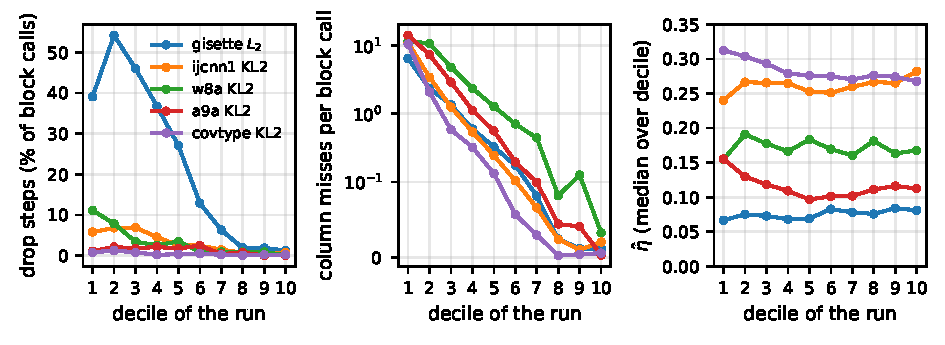
\includegraphics[width=\linewidth]{figs/fig_diag.pdf}
\caption{Along the run at $k=16$ (deciles of the iteration count, one
line per cell): fraction of block calls that are drops, column misses per
block call, and the effective correlation $\hat\eta$. Drops and misses
are paid while the support is built and become rare once it has
settled, the shape Theorem~\ref{thm:ident} describes; $\hat\eta$ is
constant along the run.}\label{fig:diag}
\end{figure}

Four facts follow.
\begin{itemize}\setlength\itemsep{0pt}
\item \emph{$\hat\eta$ is stable on each cell.} The effective
correlation does not move with $k$ nor along the run
(Figure~\ref{fig:diag}, right), although it is a statistic of the
iterates and the pairing rule rather than of the data alone; it is $0.07$ on
gisette, $0.11$ on a9a, $0.17$ on w8a, $0.26$ on ijcnn1 and $0.29$ on
covtype, and $0.004$ on the synthetic dense-support instance of
Table~\ref{tab:kabl}. The mean relative pair gain
$Q/k'=(1/k')\sum_j\Delta_j/\Delta_1$ (median $Q$ over the run's block
calls with pair 1 uncapped, divided by the mean number of retained
pairs) is $0.92$--$0.98$ at $k=4$, $0.83$--$0.98$ at $k=16$ and
$0.78$--$0.88$ at $k=32$ (Table~\ref{tab:assump} lists the $k=16$
values): the useful progress beyond the leading pair is never the
limit, the loss to combination is. The measured gain ratios (median
$\max(\Delta_B,\Delta_1)/\Delta_1$ over the same calls: $3.4/6.9/7.5$ on
gisette and $2.1/2.8/3.0$ on ijcnn1 at $k=4/16/32$) follow
$k/(1+\hat\eta(k-1))$ within $25\%$ and saturate at about $1/\hat\eta$.
\item \emph{$k^*$ is $7$--$14$ on every cell}, because $a/b$ is
$16$--$28$ throughout and $\hat\eta\in[0.07,0.29]$: a fixed block size
of $8$--$16$ is within $16\%$ of the best measured time on all five
cells ($k{=}16$ against the best size: $16\%$ on gisette, $0$--$5\%$
elsewhere), which is why the untuned $k=16$ of Section~\ref{sec:exp}
never lost to another size by more than that.
\item \emph{The wall-clock gain is bounded by the column share.} The
block cannot touch the column term of the timing model
($N_{\mathrm{cols}}$ varies by under $20\%$ across $k$ on every cell),
so its speed-up over the guarded single pair is $1.1\times$ where columns
are $93\%$ of the run (gisette), $2.2\times$ at $64\%$ (w8a),
$2.8\times$ at $41\%$ (a9a) and $1.9$--$2.1\times$ at $17\%$ (ijcnn1,
covtype), where the iteration gain has already saturated at $1/\hat\eta$.
The model's time predictions are within $10\%$ of the measurements at
$k\le4$ and on gisette; at $k=16$--$32$ on the kernel cells they are
$10$--$40\%$ too high, because the runs need fewer iterations than the
one-state ratio predicts: the trajectory effect is in the block's
favour, and the model is conservative.
\item \emph{Drops are front-loaded} (Figure~\ref{fig:diag}, left). On
gisette at $k=16$ half of the block calls in the first three deciles are
drops and $1$--$2\%$ in the last three; the kernel cells show the same
shape at lower levels; nearly every case-(b) call is a drop, so the
best-of-four branch is rare. Column misses follow the same curve, so on
column-bound cells the whole column bill is paid during identification
whichever $k$ is used. Total drops per final support point are
$0.13/0.13/0.48/0.69$ on gisette and $0.003$--$0.10$ on the kernel cells
for $k=1/4/16/32$: proportional to the support, growing with $k$, and an
order of magnitude more frequent on the sparse linear cell, where fresh
receivers of small weight become the worst donor at once.
\end{itemize}
\begin{table}[t]\centering\scriptsize
\caption{The theorem's assumptions against the measured mechanism at
$k=16$ (seed 0; \texttt{src/block\_diagnostics.py} on a second machine,
with iteration and drop counts identical to the runs of
Table~\ref{tab:diag}; its $\hat\eta$ differs from Table~\ref{tab:diag}
in the second decimal because it is the median over the all-uncapped
calls at $k=16$ only). Over the
block calls with every retained pair uncapped: median maximum absolute
pairwise cosine of the retained directions (the $\eta$ of
Proposition~\ref{prop:ratio}), median minimum relative pair gain (its
$\beta_{\mathrm{flat}}$), and the lower bound the proposition then
guarantees for the guarded ratio $\max(\Delta_B,\Delta_1)/\Delta_1$,
$(1+\beta_{\mathrm{flat}}(k'-1))/(1+\eta(k'-1))$ (column ``bound''); against
the effective correlation $\hat\eta$, the mean relative pair gain
$Q/k'$, the model ratio $k'/(1+\hat\eta(k'-1))$ and the measured median
of $\max(\Delta_B,\Delta_1)/\Delta_1$, the last three over the block
calls with pair 1 uncapped.}\label{tab:assump}
\begin{tabular}{lrrrrrrrr}\toprule
cell & all pairs uncapped & $\max|\cos|$ & $\beta_{\mathrm{flat}}$ & bound & $\hat\eta$ & $Q/k'$ & model & measured \\\midrule
gisette $L_2$ & 43\% & 0.33 & 0.53 & 1.5 & 0.08 & 0.98 & 7.4 & 6.9 \\
ijcnn1 KL2 & 73\% & 0.42 & 0.80 & 1.8 & 0.26 & 0.89 & 3.2 & 2.8 \\
w8a KL2 & 76\% & 0.33 & 0.77 & 2.1 & 0.17 & 0.88 & 4.4 & 3.6 \\
a9a KL2 & 89\% & 0.28 & 0.70 & 2.2 & 0.12 & 0.83 & 5.8 & 4.6 \\
covtype KL2 & 96\% & 0.42 & 0.82 & 1.8 & 0.28 & 0.91 & 3.0 & 2.7 \\
\bottomrule\end{tabular}\end{table}

\emph{The theorem's constants are not what the mechanism runs on.}
Table~\ref{tab:assump} records the assumptions of
Proposition~\ref{prop:ratio} on the real cells. The maximum pairwise
cosine is $0.3$--$0.4$ on every cell, so the $\eta$ of the proposition
does not distinguish the cells at all, whereas the effective correlation
$\hat\eta$ spans $0.07$--$0.29$ and does; the minimum relative gain is
$0.5$--$0.8$; and at $k=16$ only $43$--$96\%$ of the block calls have all
pairs uncapped, so the proposition applies to a minority of the calls on
gisette. The lower bound the proposition guarantees for the guarded
ratio from these constants is $1.5$--$2.2$, against measured medians of
$2.7$--$6.9$ (the bound is an inequality, so the gap is slack, not a
contradiction); the exact
identity $Q/\chi$ (the ``model'' column) reproduces the measurement
because it uses the $\gamma$-weighted aggregate in which the cross terms
largely cancel, not the worst pair. The right reading of
Proposition~\ref{prop:ratio} is therefore its first, exact, half; the
$\eta$-diverse, $\beta_{\mathrm{flat}}$-flat bound is a worst case that real blocks beat
by a factor of $1.5$--$4.6$.

The measurements are from one seed per cell and the fits are
retrospective (the coefficients are estimated from the same four runs
they describe); the ratios they support (Tables~\ref{tab:kreal}
and~\ref{tab:bpcg}) are reproduced across three seeds in isolated runs,
and Section~\ref{sec:adaptive} is the prospective test. On the
identification mechanism the figure is consistent with
Theorem~\ref{thm:ident} but does not verify it: the theorem's thresholds
$H_{\mathrm{id}},H_{\mathrm w}$ lie far below the stopping tolerance of
these runs, and late drops, though rare, do occur. Section~\ref{sec:ident-check}
tests the theorem where its constants can be computed.

\subsection{An adaptive block size}\label{sec:adaptive}

Every quantity in \eqref{eq:kstar} is observable while the solver runs:
$\chi$ is computed by the guard at every block step, so
$\hat\eta=(\chi-1)/(k'-1)$ costs nothing, and $a/b$ is a property of
the implementation ($16$--$28$ in Table~\ref{tab:diag}). The released
code therefore offers \texttt{block\_size='auto'}: every $50$ iterations
it sets $k$ to $\sqrt{(a/b)(1-\hat\eta)/\hat\eta}$, clipped to $[1,k_{\max}]$,
with $\hat\eta$ the median over the window's block steps with $k'>1$
(when fewer than five such steps exist, as at $k=1$, the rule doubles
$k$ to obtain a signal; a non-positive $\hat\eta$ is floored at $10^{-3}$
before the square root, which sends $k$ to $k_{\max}$), and halves $k$ instead when
more than $10\%$ of the window's block calls had their leading pair
capped (drops are outrunning the support). Guard and fallback are
untouched, so Theorem~\ref{thm:linear} applies with $k_{\max}$ in the
drop bound. What is prospective and what is not should be stated
precisely. The rule, its window, $k_{\max}=32$ and the ratio $a/b=20$
were fixed from the two pilot cells (gisette, ijcnn1) before w8a, a9a
and covtype were run at all; on a run the rule reads only its own
window's $\chi$ values, never the per-cell $\hat\eta$ of
Table~\ref{tab:diag}, which is a retrospective median over three
complete runs and enters nothing but the fitted $k^*$ column of that
table. The test of the rule is therefore the wall-clock it achieves on
the three held-out cells against the fixed sizes run under the same
protocol (Table~\ref{tab:kreal}); the agreement of the sizes it chose
($10$ on w8a, $13$ on a9a, $7$ on covtype) with the retrospectively
fitted $k^*$ ($9$, $13$, $8$) is a consistency check of the model, not
the test. On
the two pilot cells (Table~\ref{tab:kreal}) it settles at $k{=}9$ then
$15$ on gisette, tying the fixed sizes within CI, and at $k{=}7$--$8$ on
ijcnn1, where it is the fastest configuration ($4.7\pm0.6$\,s against
$5.3\pm0.8$\,s for $k{=}16$). On the three held-out cells
(Table~\ref{tab:kreal}, three seeds, isolated) it settles at $k=10$,
$13$ and $7$ and takes $3.8\pm0.2$, $10.0\pm0.5$ and $16.8\pm1.7$\,s
against $4.0\pm0.2$, $10.0\pm0.5$ and $17.4\pm0.5$\,s for the best fixed
size tested, $k{=}16$: it ties or beats it on every held-out cell,
which is the prospective test the model had to pass. Table~\ref{tab:adaptive} tests it where
$\eta$ actually varies: synthetic $L_2$ instances ($n{=}2{,}000$ per
class, $C{=}1$) whose transfer directions decorrelate as the dimension
grows, so that $\hat\eta$ falls from $0.31$ at $d{=}20$ to $0.001$ at
$d{=}1{,}000$. The rule tracks $k^*$ across two orders of magnitude of
$\hat\eta$ and matches the best fixed size within the resolution of these
short single-seed runs (about $0.1$\,s) at every~$d$.

\begin{table}[t]\centering\scriptsize
\caption{Adaptive block size on synthetic $L_2$ instances of varying
directional diversity (one process, seed 0, $a/b$ set to $20$,
$k_{\max}=32$). Times for guarded $k{=}1$ and fixed $k=4/16/32$; ``auto''
reports the size the rule settled on and its time.}\label{tab:adaptive}
\begin{tabular}{rrrrrrrr}\toprule
$d$ & $\hat\eta$ & $k^*$ & $k{=}1$ (s) & $k{=}4$ & $k{=}16$ & $k{=}32$ & auto: $k$, time (s) \\\midrule
20 & 0.31 & 7 & 1.3 & 1.0 & 1.1 & 1.3 & 6, 1.1 \\
50 & 0.10 & 13 & 2.1 & 1.2 & 1.0 & 1.3 & 12, 1.1 \\
100 & 0.03 & 25 & 3.5 & 1.8 & 1.1 & 1.2 & 24, 1.1 \\
300 & 0.00 & $>32$ & 1.7 & 0.7 & 0.4 & 0.4 & 32, 0.4 \\
1,000 & 0.00 & $>32$ & 1.5 & 0.9 & 0.7 & 0.7 & 32, 0.7 \\
\bottomrule\end{tabular}\end{table}

\subsection{Numerical check of Theorem~\ref{thm:ident}}\label{sec:ident-check}

The theorem's constants are computable on small instances. For $40$
random hard-margin instances ($d=4$, ten points per class, Gaussian
clouds $2.5$ apart) the SLSQP reference gives $z^*$, the faces, $\tau$,
$\alpha_{\min}$, $d_{\min}$ and $\sigma$ (as the singular value of
Assumption~\ref{ass:nondeg}); $12$ instances that fail strict
complementarity or affine independence within $10^{-7}$ are skipped, and
the remaining $28$ are run with $k\in\{1,4,16\}$ to certificate tolerance $\varepsilon=10^{-10}$
with both supports snapshotted at every iteration
(\texttt{src/ident\_check.py}, $84$ runs). Three things are checked. The
weight inequality (F2), $\omega_t\le h_t/\tau$, holds at every iteration
of every run. From the first iteration at which the proof's radius and
weight conditions hold (the conditions on $\varrho_t$, $\omega_t$ and
$2h+R\sqrt{2h}$ that define $H_{\mathrm{id}}$ and $H_{\mathrm w}$),
claims (i) and (ii) hold to the end of every run: every removal of a
non-face point is a drop, no non-face point enters, and after
$t_1$ no index leaves. The third finding is that those conditions
engage far later than the mechanism they certify. The last non-face
support point leaves, and the last drop occurs, at $h\approx10^{-3}$
(median; $h_0\approx6$); the proof's conditions first hold at
$h\approx3\times10^{-13}$, and the sufficient $h$-thresholds
$H_{\mathrm{id}},H_{\mathrm w}$ lie at $3\times10^{-18}$. The theorem is
therefore verified in its ingredients and contradicted nowhere, but its
thresholds are pessimistic by some $14$ orders of magnitude in $h$
(about $7$ in $\norm{z-z^*}$) on these instances, most of it in the
passage from $r$ to $h$ through $r^2\le(4R^2/\delta^*)\sqrt{2h}$. The
large-data profiles of Figure~\ref{fig:diag} are consistent with the
mechanism; they do not verify the thresholds, which no run of
Section~\ref{sec:exp} reaches.
